\documentclass{beamer}
\usepackage[utf8]{inputenc}
\usepackage{pre}
\usetheme{Madrid}
\usecolortheme{default}
\setbeamertemplate{bibliography item}[text]
\bibliographystyle{plain}

\title[Final project] 
{Group Final project: Baseline Implementation and Investigation}

\author{8-Hengke Jiang, 13-Yuting Jiang, 20-Rock, 30-Ethan, 35-Jade Lin}

% \institute[] % (optional)
% { 
%   {linyh63@mail2.sysu.edu.cn}
% }

\date[7.7.2024] % (optional)

\AtBeginSection[]
{
  \begin{frame}
    \frametitle{Table of Contents}
    \tableofcontents[currentsection]
  \end{frame}
}

\begin{document}
\frame{\titlepage}
% \tableofcontents
\section{Text classification and dataset}
\begin{frame}
  \frametitle{Text classification}
  Why Text classification is still alive?
\end{frame}
\begin{frame}
  \frametitle{Text classification applications}
  \begin{itemize}
    \item Customer Support and Feedback Analysis: Automatically classifying customer queries into categories like technical support, billing issues, product inquiries, etc;
    \item Content Moderation and Filtering: Filtering and moderating user-generated content on social media platforms, forums, and online communities;
    \item Information Retrieval: Improving search engine results by categorizing and organizing documents or web pages based on their topics or relevance;
    \item Filtering incoming emails to separate spam or junk emails from legitimate messages;
  \end{itemize}
\end{frame}
\begin{frame}
  \frametitle{Text classification}
  \begin{figure}[H]
    \centering
    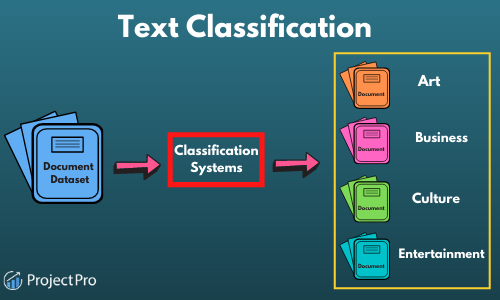
\includegraphics[width=7cm]{pictures/Text_Classification_Machine_Learning_NLP.png}
  \end{figure}
  \begin{itemize}
    \item News Categorization: Organizing news articles and updates into different categories or topics for readers.
  \end{itemize}
\end{frame}
\begin{frame}{AG News}
  \frametitle{Dataset and SOA}
  \begin{itemize}
    \item 120,000 training articles, 7600 testing articles;
    \item Categories divided: World, Sports, Business, Science/Technology
    \item Format: Each article is represented as a text string along with its corresponding label indicating the topic category.
  \end{itemize}
  \begin{figure}[H]
    \centering
    \includegraphics[width=11cm]{D:/Pictures/Screenshots/屏幕截图 2024-07-07 205959.png}
  \end{figure}
\end{frame}
\section{BERT and modified BERT}
\begin{frame}
  \frametitle{BERT}
  Base on encoder part of transformer\cite{vaswani2023attentionneed}, BERT(Bidirectional Encoder Representations from Transformers)\cite{devlin2019bertpretrainingdeepbidirectional} is developed to do tasks as: 
  
  Text classification, Question Answering, Text Generation, Language Understanding, and Sentence Embeddings.
  \begin{figure}[H]
    \centering
    \includegraphics[width=7cm]{D:/Pictures/Screenshots/屏幕截图 2024-07-07 175555.png}
  \end{figure}
  Attention: without decoder part, BERT is not used for translation.
\end{frame}
\begin{frame}{Feature of BERT-base}
  \begin{itemize}
    \item 30,000 token vocabulary
    \item Transformer Blocks: 12 layers;
    \item Hidden Size: 768 (number of units in the hidden layers);
    \item Attention Heads: 12
    \item Number of parameters: 110M
  \end{itemize}
  \begin{figure}[H]
    \centering
    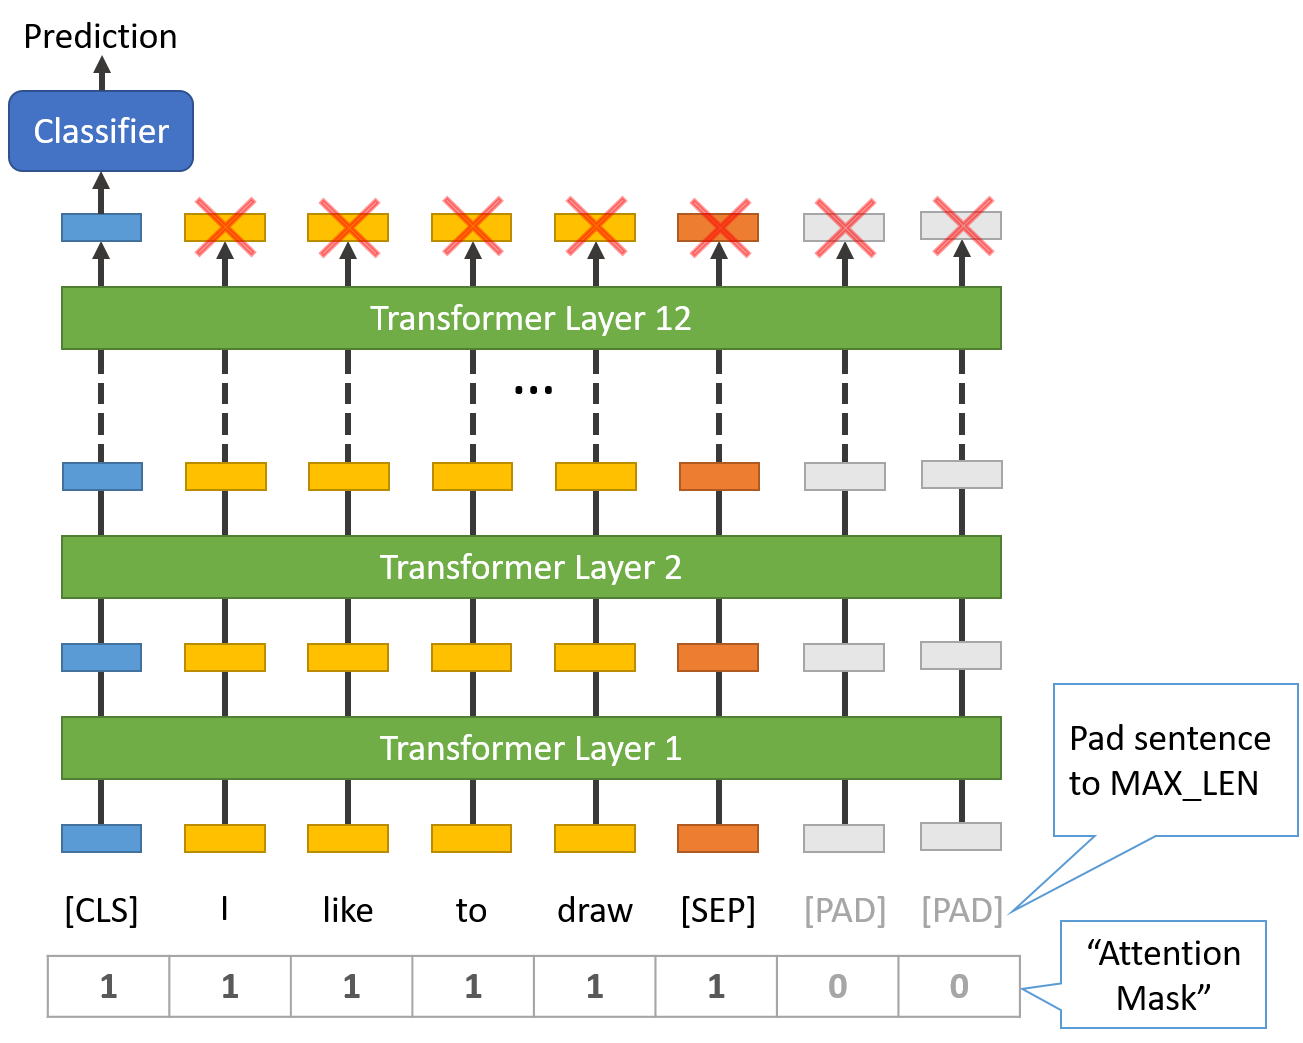
\includegraphics[width=6cm]{pictures/padding_and_mask.png}
  \end{figure}
\end{frame}
\begin{frame}{Modified BERT: ALBERT}
  ALBERT: a lite BERT for self-supervised learning of language representations\cite{lan2020albertlitebertselfsupervised}.

  Motivation: at some point fur-
  ther model increases become harder due to GPU/TPU memory limitations and
  longer training times. Improve BERT in 2 ways with the same number of parameters(110M).
  \begin{itemize}
    \item Tech 1: Decomposing
    the large vocabulary embedding matrix into two small matrices to separate the size of the hidden
    layers from the size of vocabulary embedding.
  \end{itemize}
  \begin{figure}[H]
    \centering
    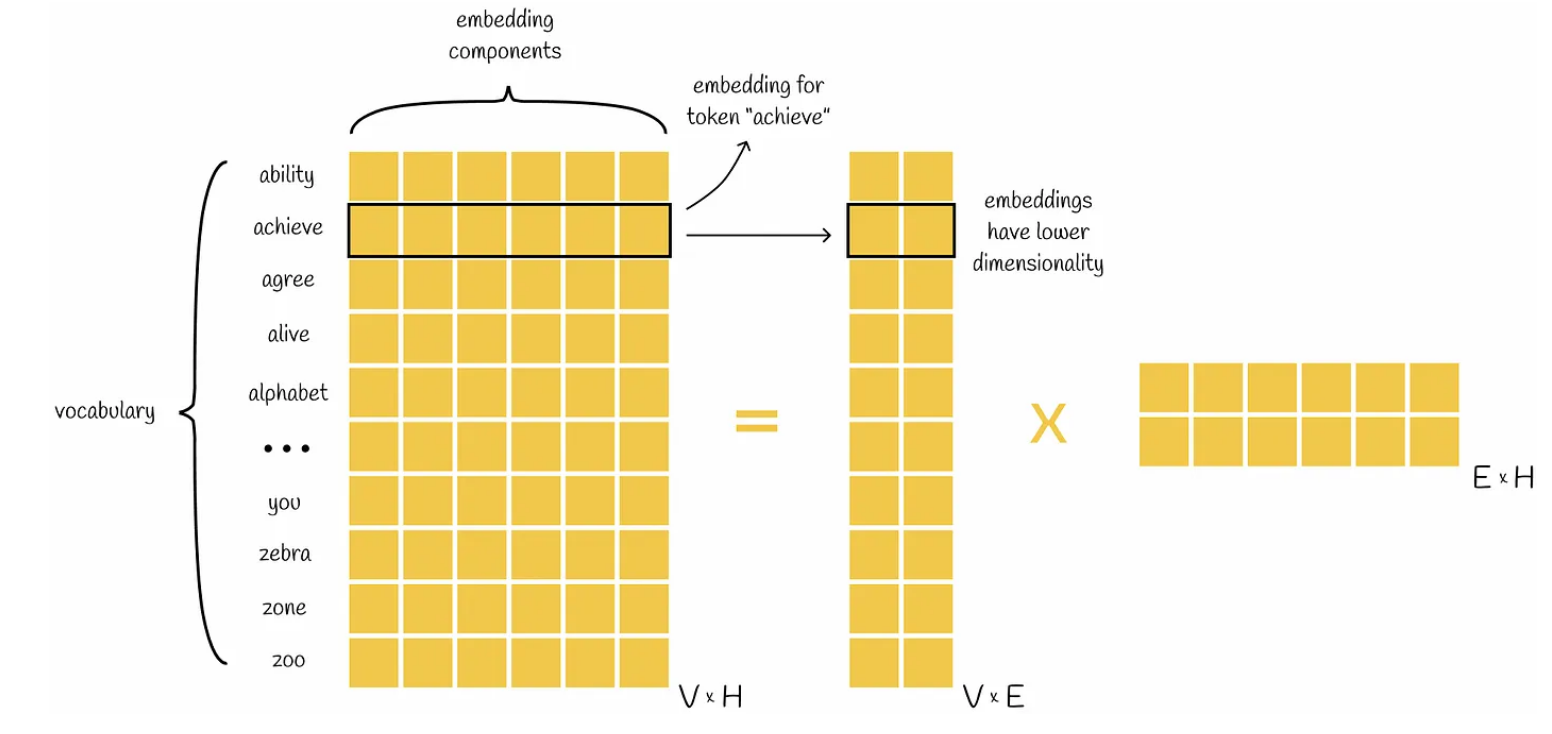
\includegraphics[width=10cm]{pictures/albert1.png}
  \end{figure}
\end{frame}
\begin{frame}{Modified BERT: ALBERT}
  \begin{itemize}
    \item Tech 2: cross-layer parameter sharing prevents the parameter from growing with the depth of the network;
  \end{itemize}
  \begin{figure}[H]
    \centering
    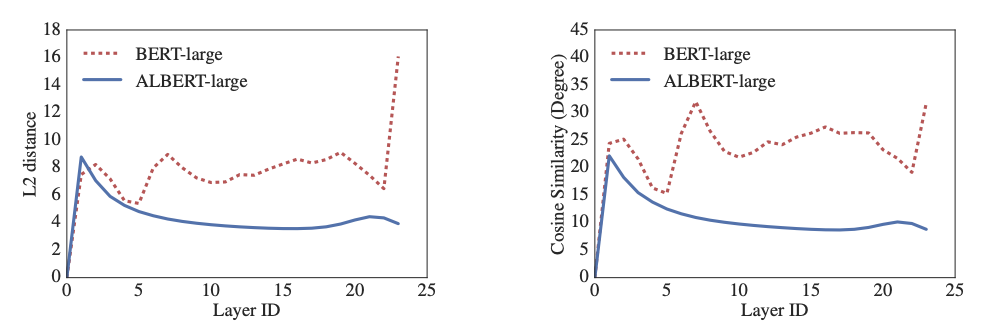
\includegraphics[width=10cm]{pictures/albert2.png}
  \end{figure}
\end{frame}
\begin{frame}{Modified BERT: ALBERT}
  \begin{figure}[H]
    \centering
    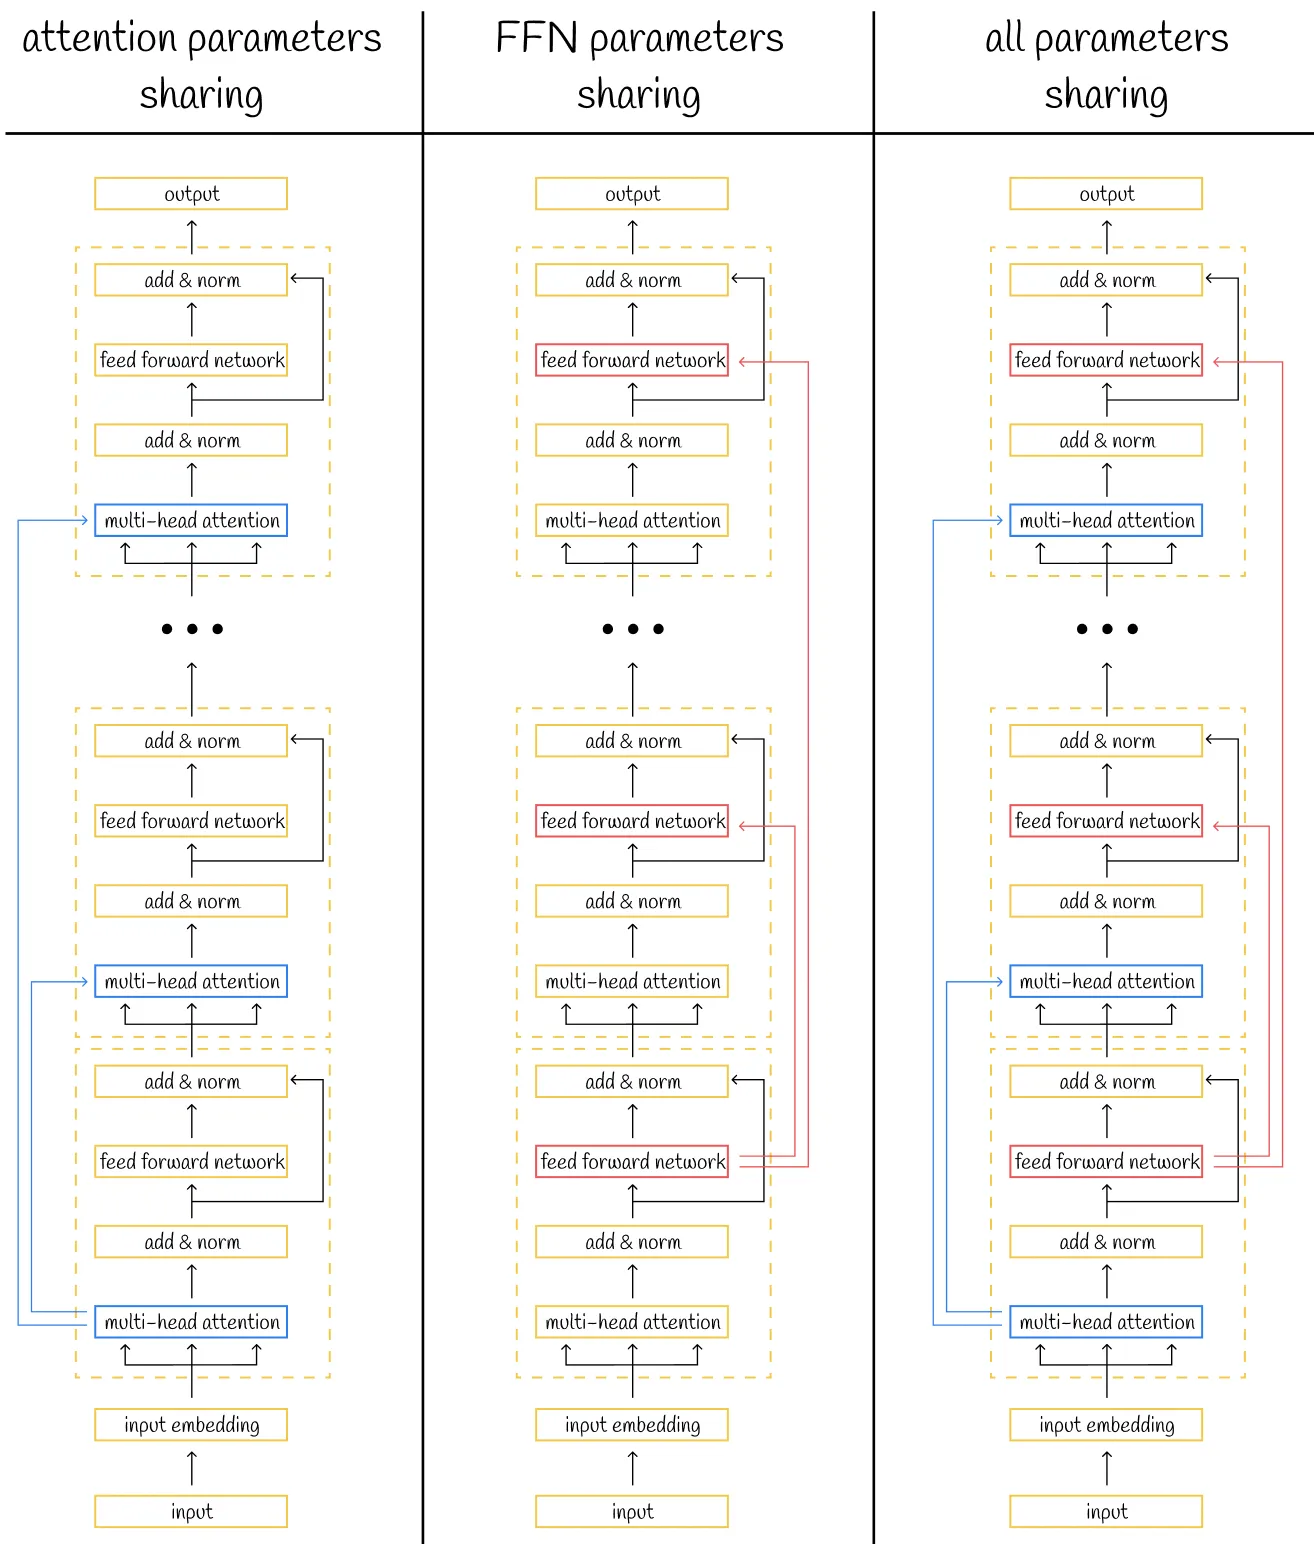
\includegraphics[width=6.5cm]{pictures/albert3.png}
  \end{figure}
\end{frame}
\begin{frame}{Modified BERT: DEBERTA}
DeBERTa: Decoding-enhanced BERT with Disentangled Attention\cite{he2021debertadecodingenhancedbertdisentangled}

Motivation: Improvement with the number of parameters close to BERT(89M vs. 110M) in two ways.
\begin{itemize}
  \item 1. Disentangled attention: Each word is represented using two vectors that encode its content and position, respectively, and the
  attention weights among words are computed using disentangled matrices based on their contents
  and relative positions, respectively. 
\end{itemize}
  \begin{figure}[H]
    \centering
    \includegraphics[width=11cm]{D:/Pictures/Screenshots/屏幕截图 2024-07-07 200140.png}
  \end{figure}
\end{frame}
\begin{frame}{Modified BERT: DEBERTA}
  \begin{itemize}
    \item 2. Enhanced mask decoder: Each word in
    DeBERTa is represented using two vectors that encode its content and position, respectively, and the
    attention weights among words are computed using disentangled matrices based on their contents
    and relative positions, respectively. 
   \end{itemize} 
  \end{frame}
\section{Implement and result}
\begin{frame}{parameter and devices(pretrained)}
  \begin{itemize}
    \item number of epoches = 6, batchsize = 32;
    \item divide training set into 2 part and shuffles, each epoch cost 4$\sim$8 min;
    \item optimizer: AdamW, with linearly decreasing learning rate(6e-5 $\sim$ 1e-5)
    \item 3 models implement.
  \end{itemize}
    \begin{figure}[H]
      \centering
      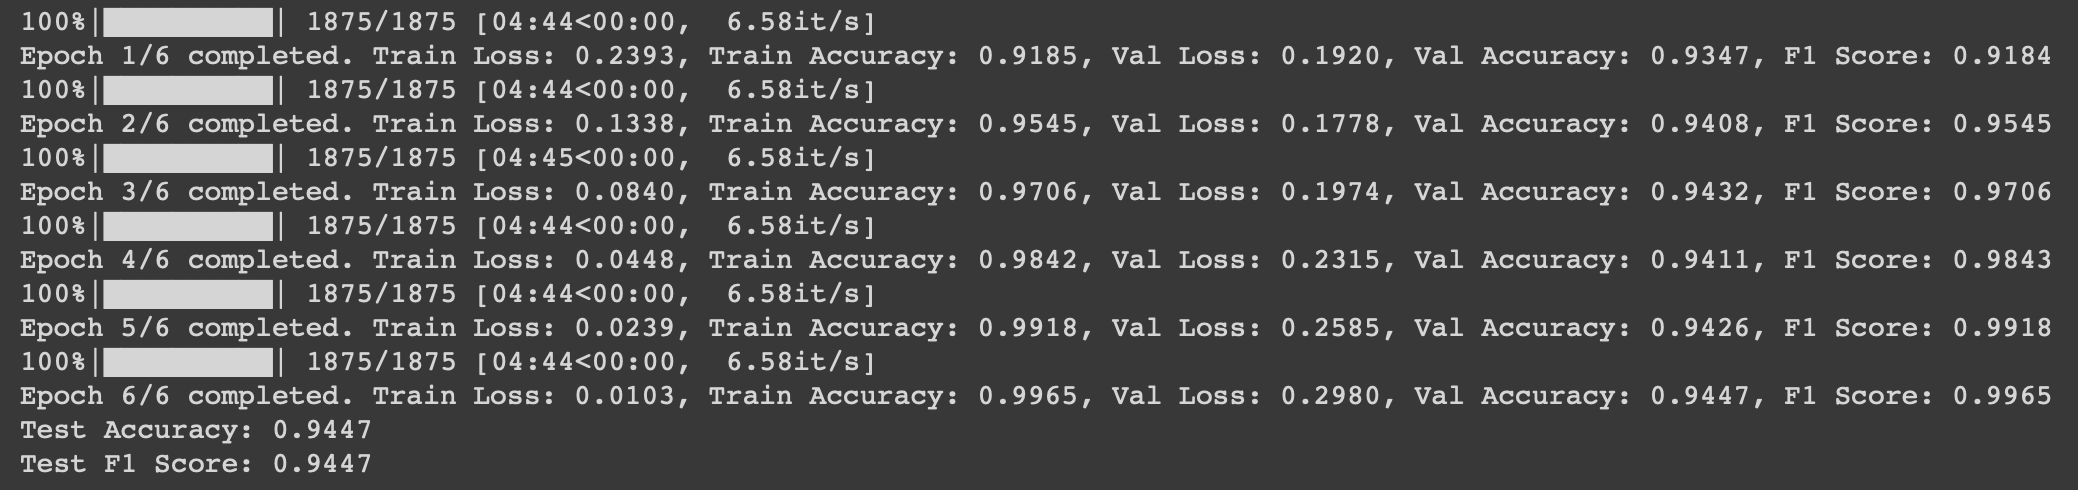
\includegraphics[width=6cm]{pictures/bertrun.png}
    \end{figure}
    \begin{figure}[H]
      \centering
      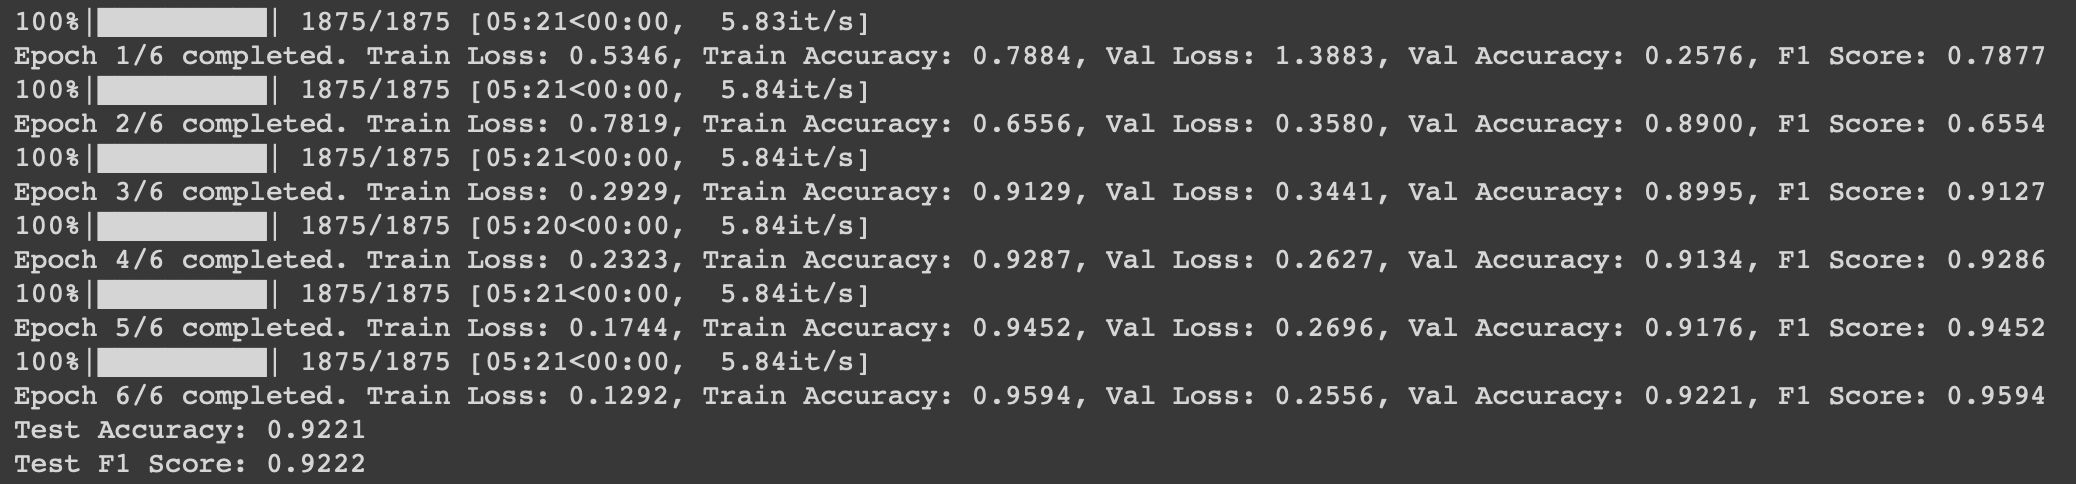
\includegraphics[width=6cm]{pictures/albertrun.png}
    \end{figure}
    \begin{figure}[H]
      \centering
      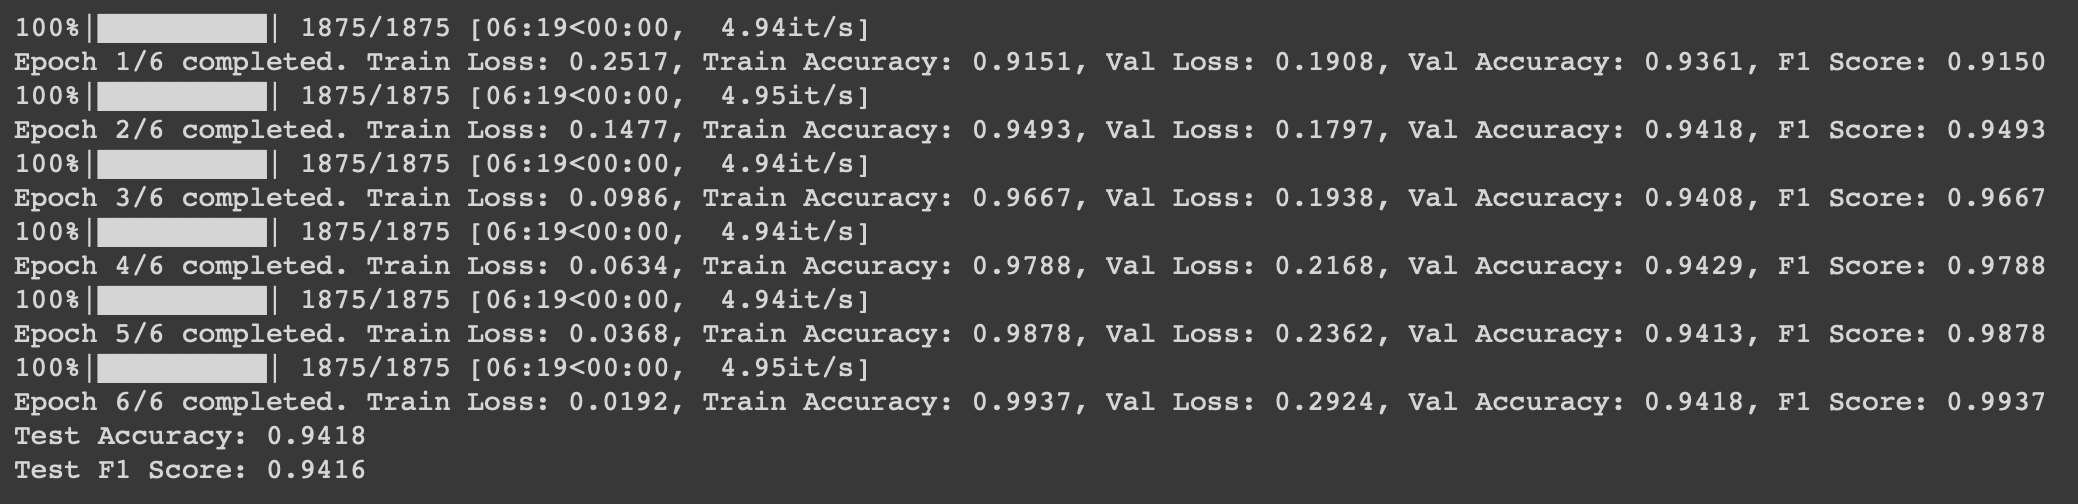
\includegraphics[width=6cm]{pictures/debertarun.png}
    \end{figure}
\end{frame}
\begin{frame}{BERT}
  \begin{figure}[H]
    \centering
    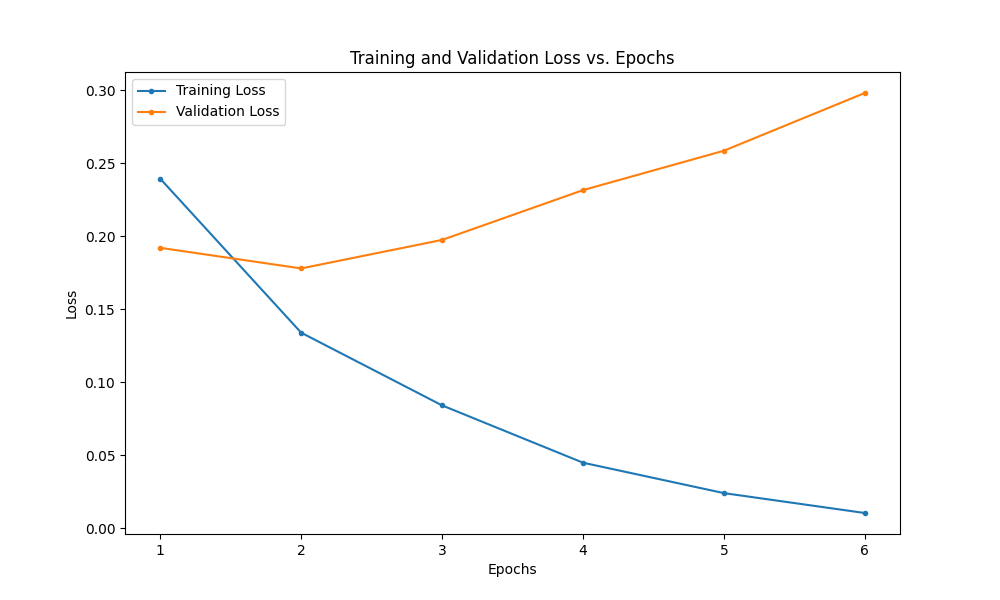
\includegraphics[width=5cm]{pictures/BERT/BERTloss_curve.png}
  \end{figure}
  \begin{figure}[htbp]
    \centering
    \begin{minipage}{0.49\linewidth}
      \centering
      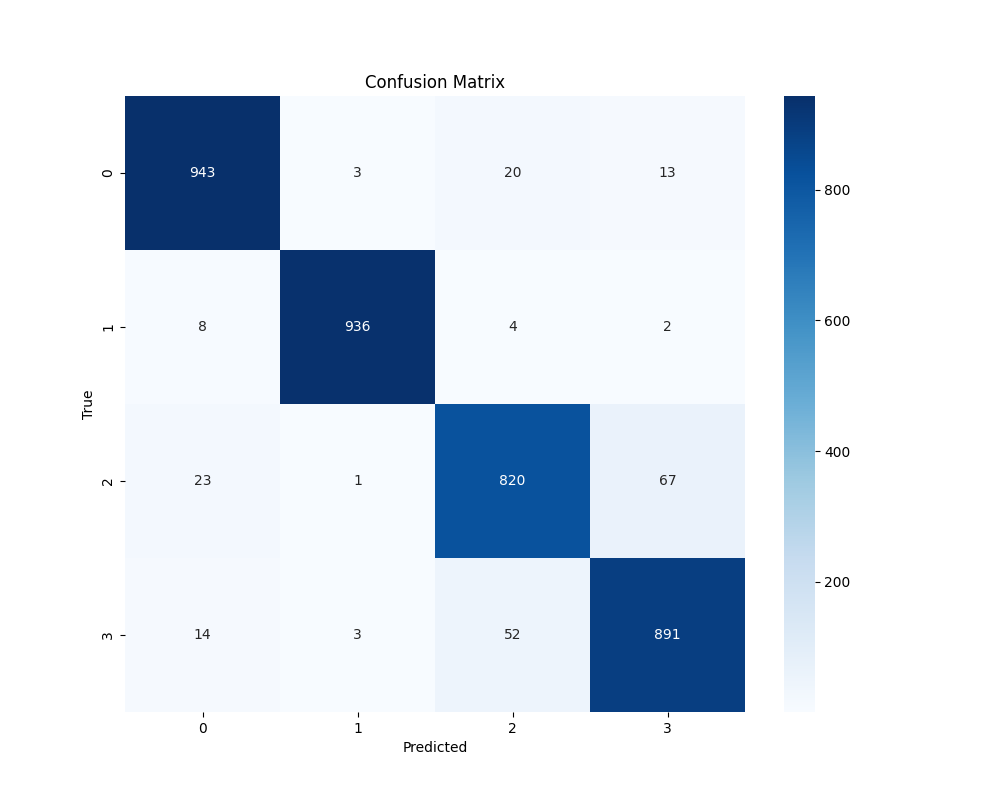
\includegraphics[width=0.9\linewidth]{pictures/BERT/BERTconfusion_matrix.png}
    \end{minipage}
    %\qquad
    \begin{minipage}{0.49\linewidth}
      \centering
      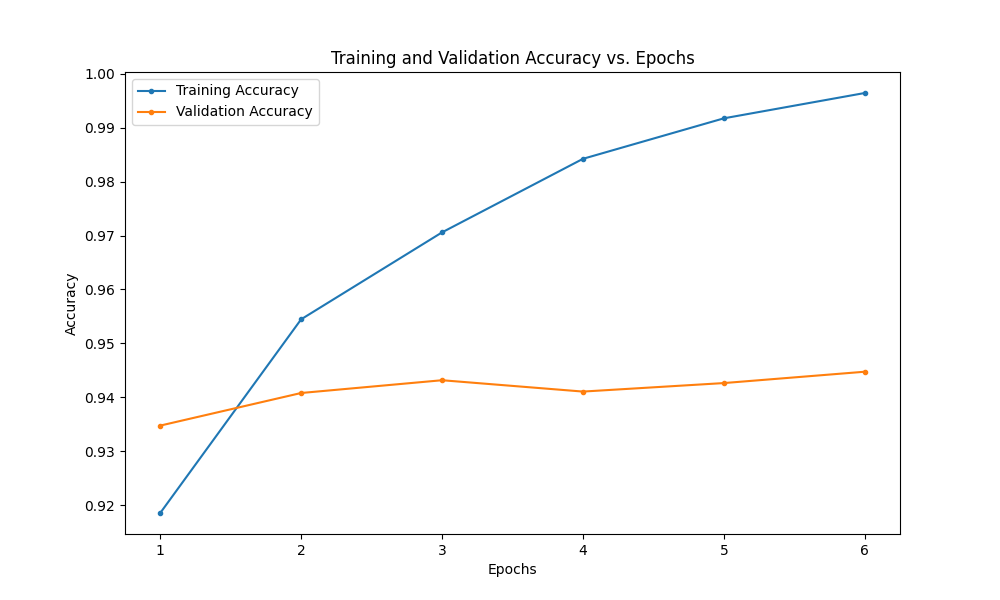
\includegraphics[width=0.9\linewidth]{pictures/BERT/BERTaccuracy_curve.png}
    \end{minipage}
  \end{figure}
\end{frame}
\begin{frame}{ALBERT}
  \begin{figure}[H]
    \centering
    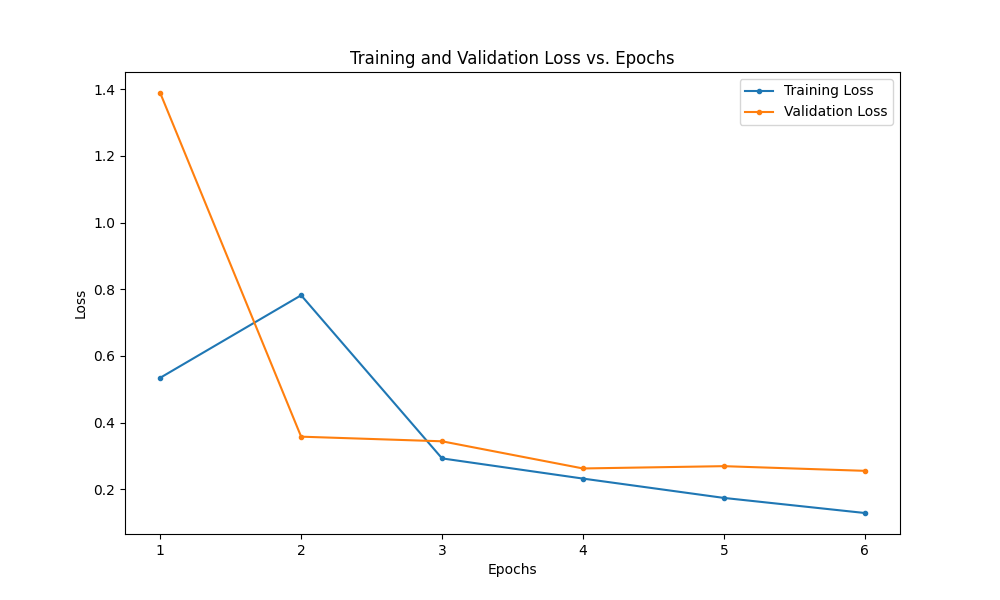
\includegraphics[width=5cm]{pictures/ALBERT/albert-v2loss_curve.png}
  \end{figure}
  \begin{figure}[htbp]
    \centering
    \begin{minipage}{0.49\linewidth}
      \centering
      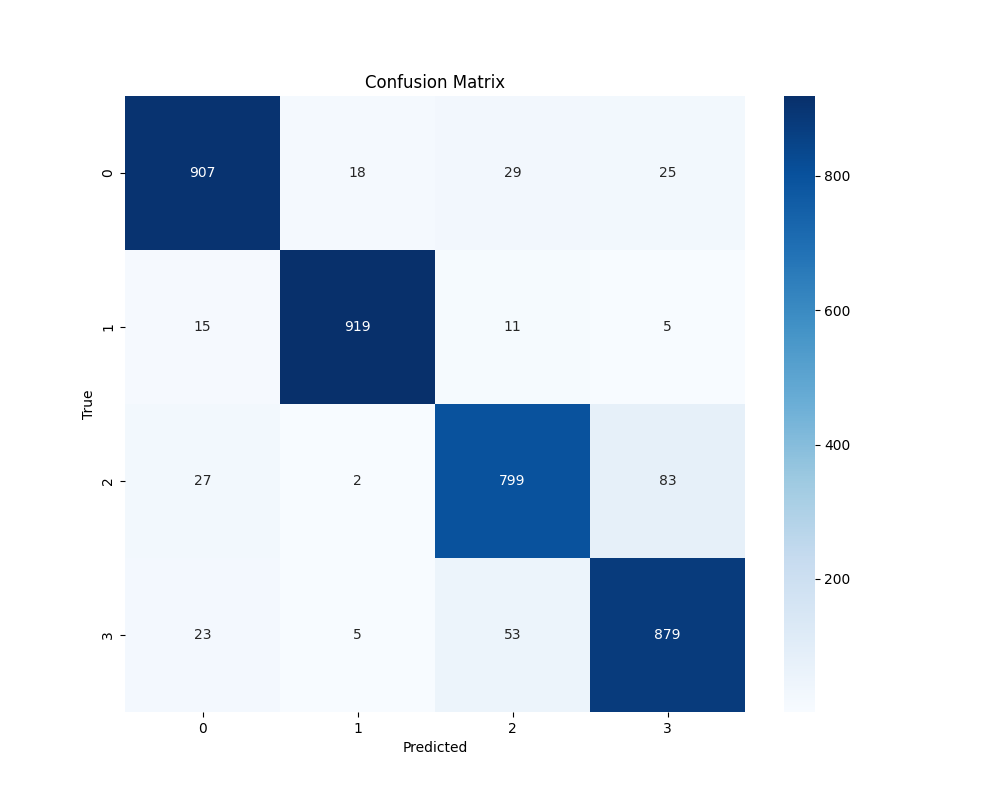
\includegraphics[width=0.9\linewidth]{pictures/ALBERT/albert-v2confusion_matrix.png}
    \end{minipage}
    %\qquad
    \begin{minipage}{0.49\linewidth}
      \centering
      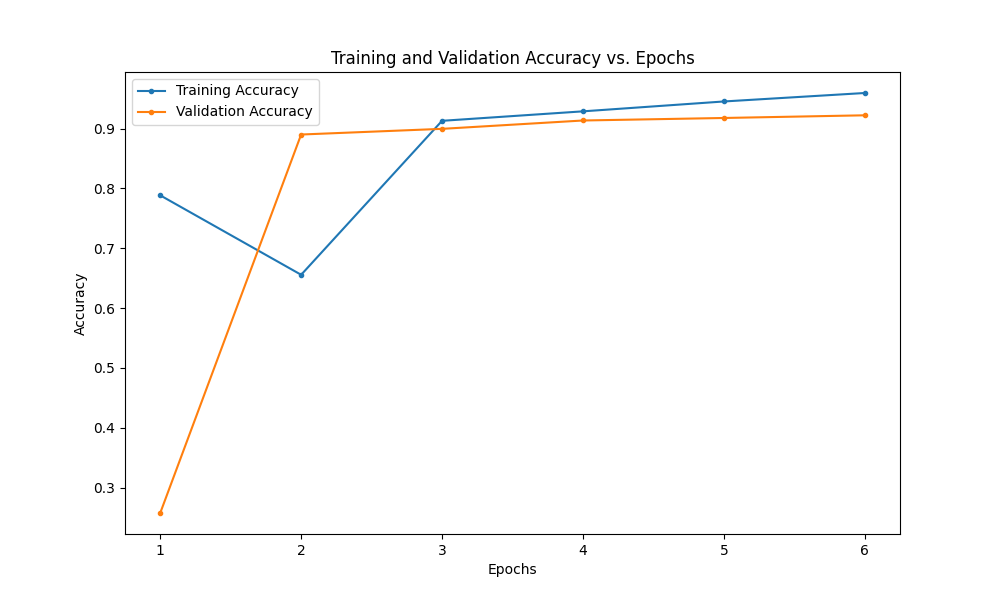
\includegraphics[width=0.9\linewidth]{pictures/ALBERT/albert-v2accuracy_curve.png}
    \end{minipage}
  \end{figure}
\end{frame}
\begin{frame}{DEBERTA}
  \begin{figure}[H]
    \centering
    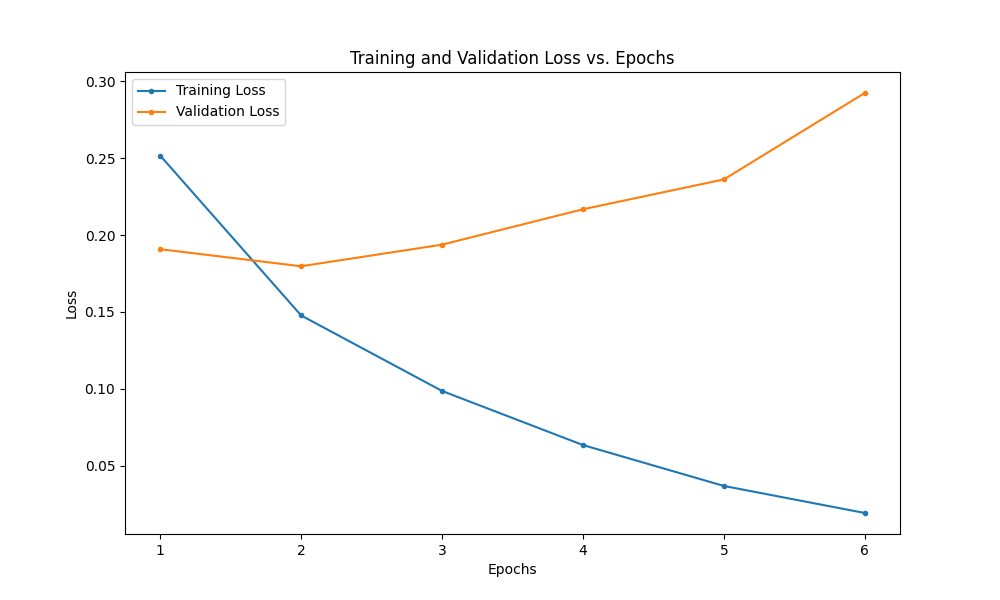
\includegraphics[width=5cm]{pictures/DeBERTa/deberta-v2loss_curve.png}
  \end{figure}
  \begin{figure}[htbp]
    \centering
    \begin{minipage}{0.49\linewidth}
      \centering
      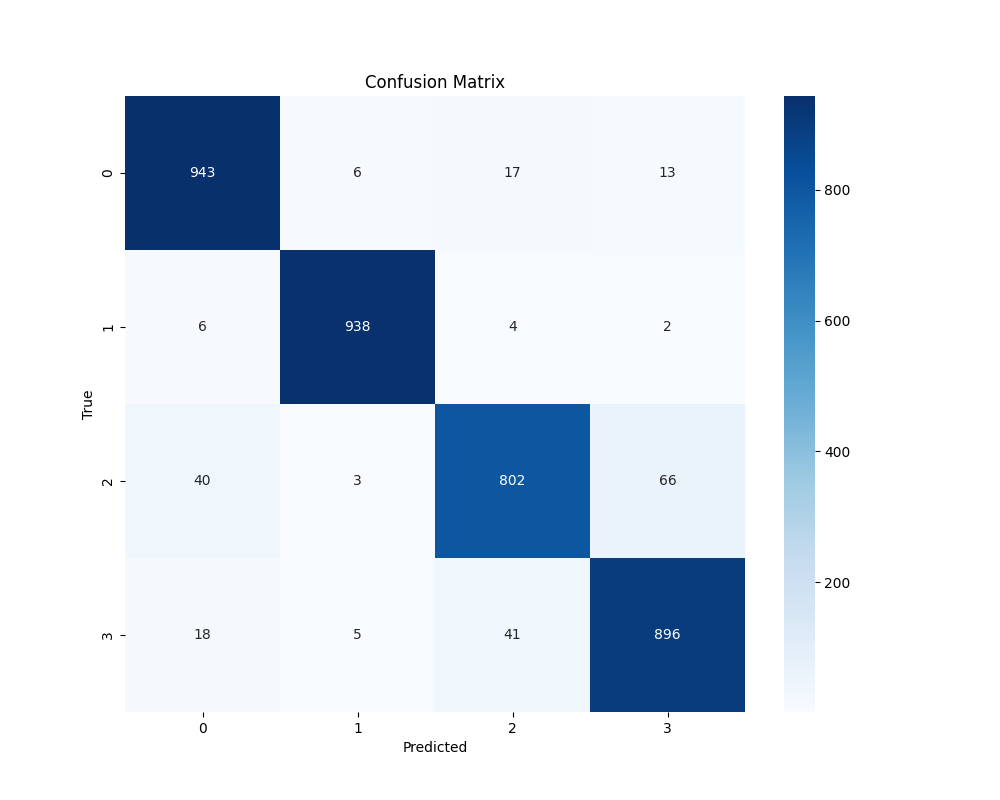
\includegraphics[width=0.9\linewidth]{pictures/DeBERTa/deberta-v2confusion_matrix.png}
    \end{minipage}
    %\qquad
    \begin{minipage}{0.49\linewidth}
      \centering
      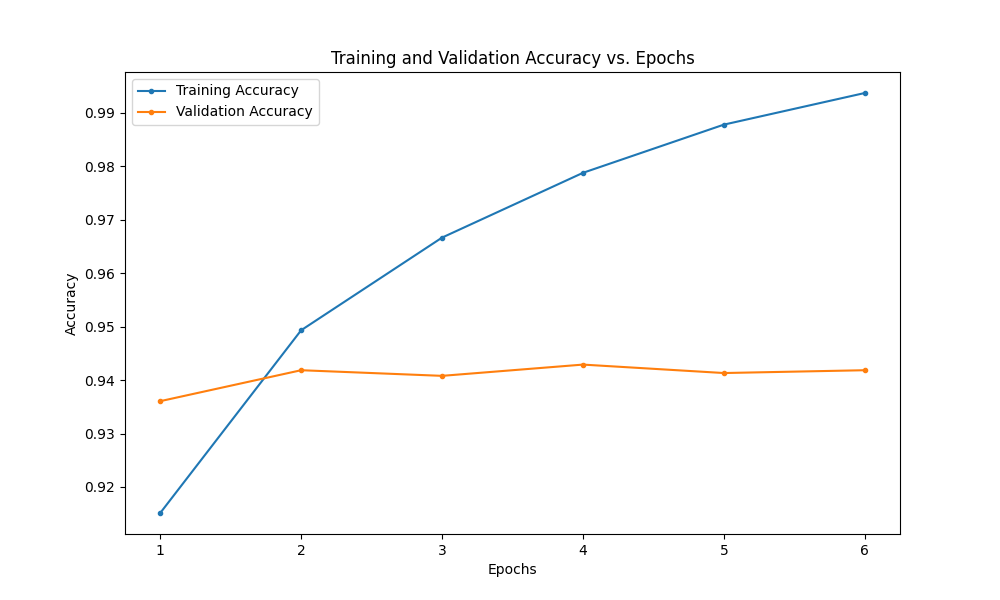
\includegraphics[width=0.9\linewidth]{pictures/DeBERTa/deberta-v2accuracy_curve.png}
    \end{minipage}
  \end{figure}
\end{frame}
\begin{frame}
  Summarazie: BERT > ALBERT > DeBERTa, partly becanse testing part is divided along with training part.
  \begin{figure}[H]
    \centering
    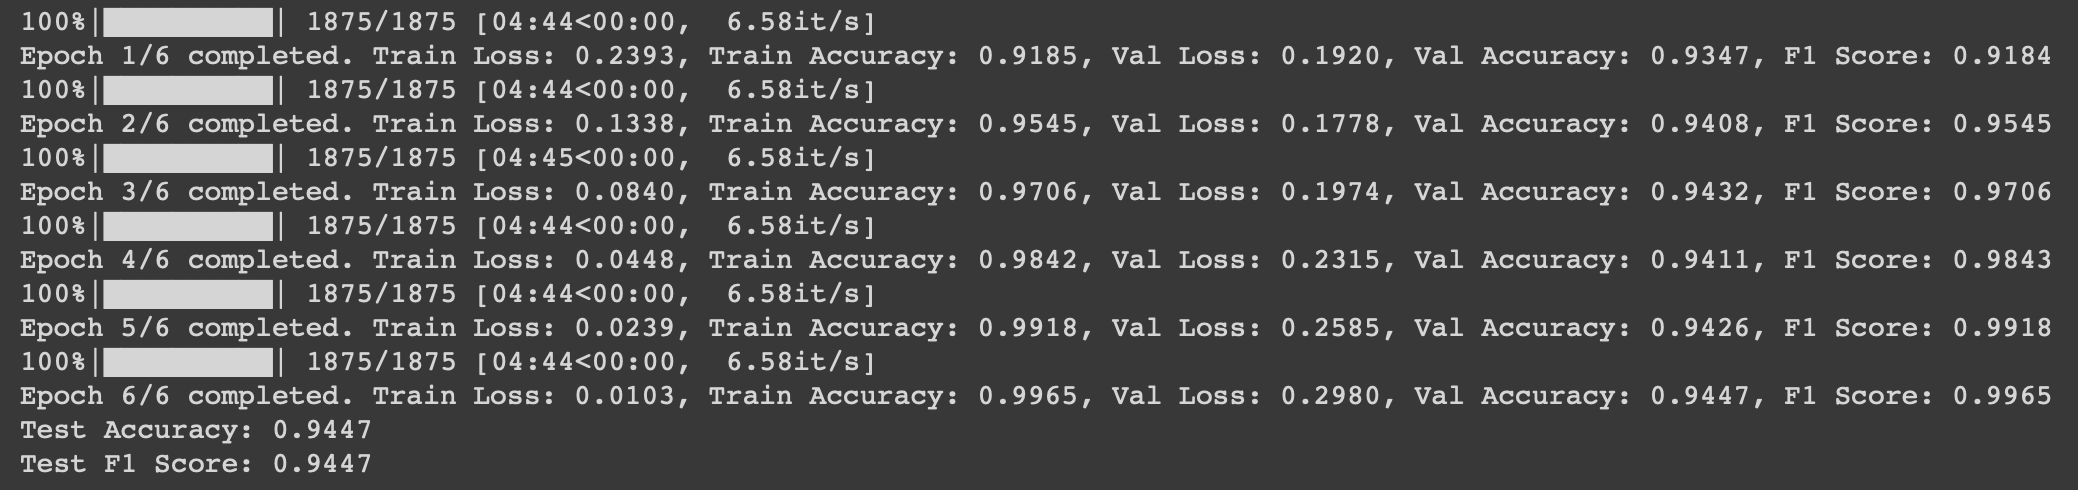
\includegraphics[width=6cm]{pictures/bertrun.png}
  \end{figure}
  \begin{figure}[H]
    \centering
    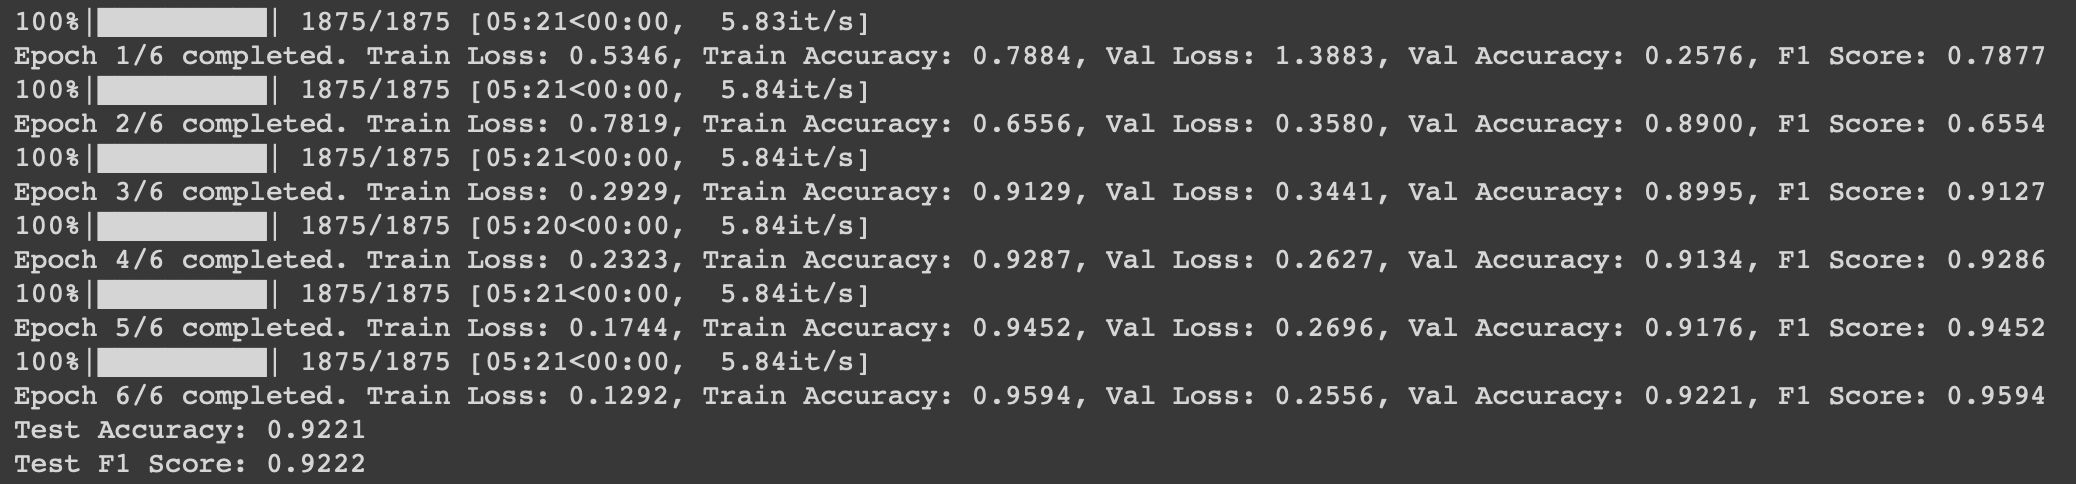
\includegraphics[width=6cm]{pictures/albertrun.png}
  \end{figure}
  \begin{figure}[H]
    \centering
    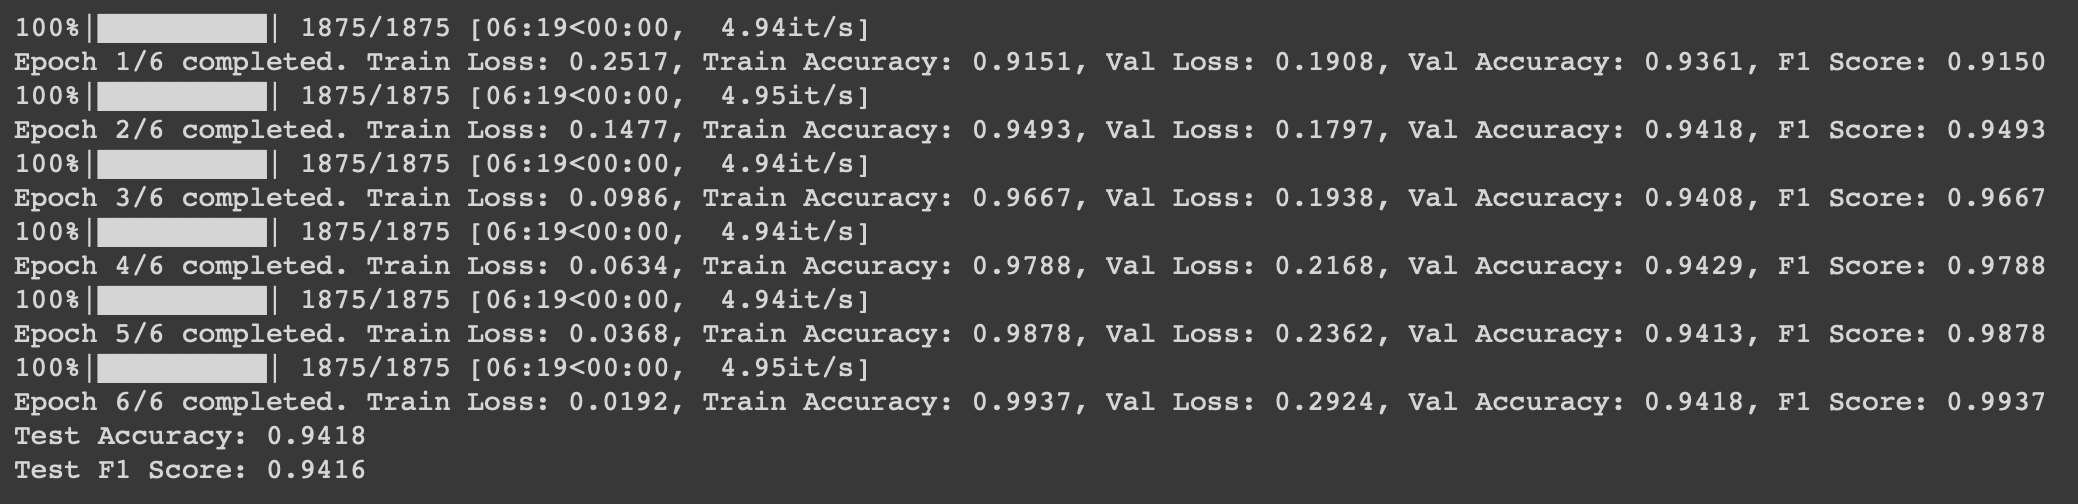
\includegraphics[width=6cm]{pictures/debertarun.png}
  \end{figure}
\end{frame}
\begin{frame}{Implement without pretrain}
  \begin{figure}[H]
    \centering
    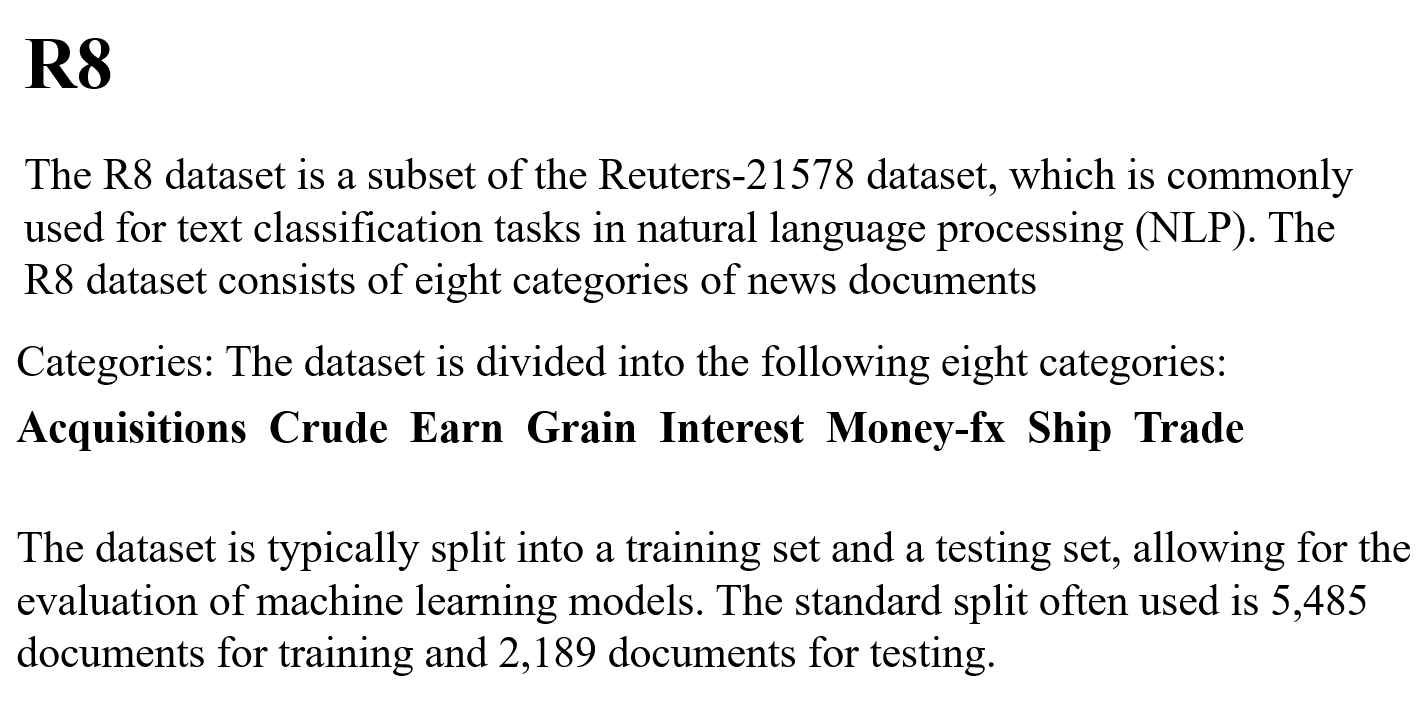
\includegraphics[width=11cm]{pictures/R8.png}
  \end{figure}
  \begin{itemize}
    \item smaller than AG News, affordable;
  \end{itemize}
\end{frame}
\begin{frame}{Implement without pretrain}
  \begin{itemize}
    \item number of epoch = 10, batchsize = 4(for time saving)
  \end{itemize}
  \begin{figure}[H]
    \centering
    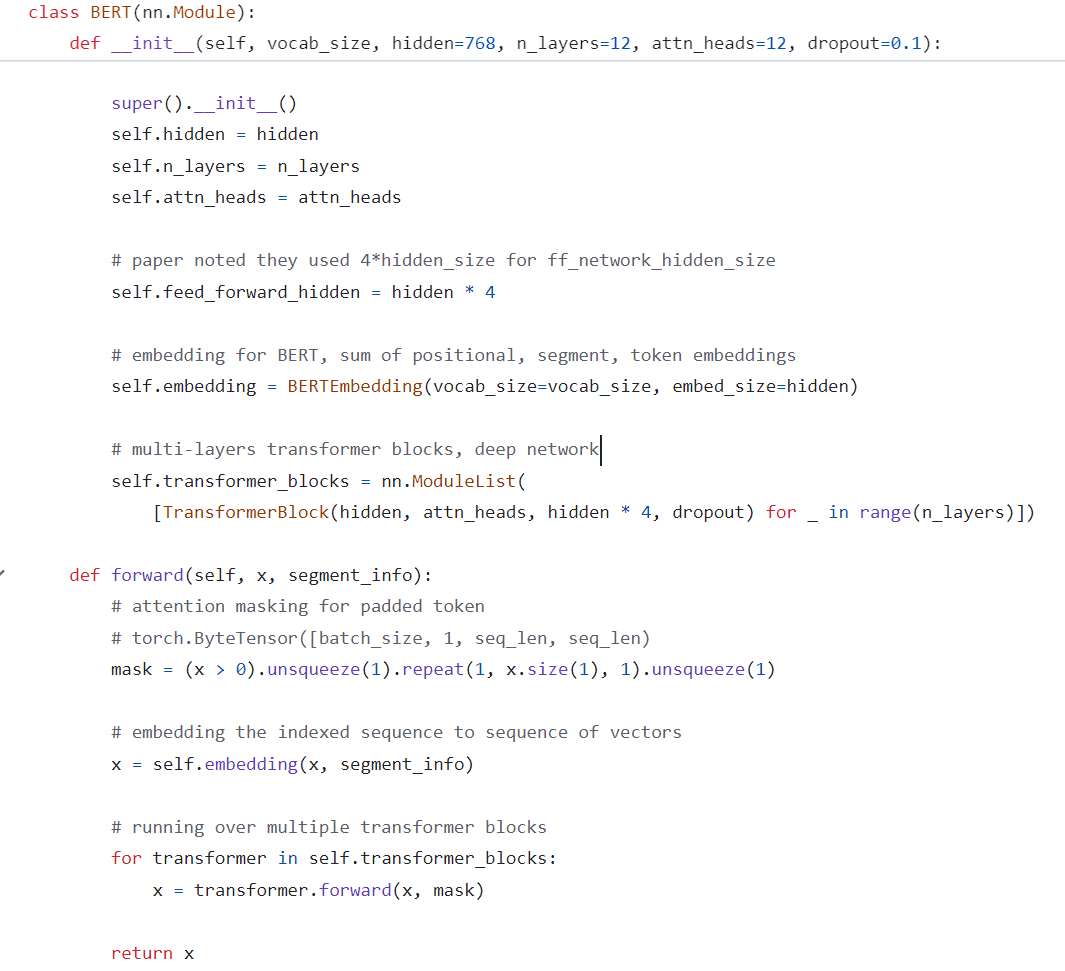
\includegraphics[width=6cm]{pictures/withoutpre.png}
  \end{figure}
\end{frame}
\begin{frame}
  \begin{figure}[htbp]
    \centering
    \begin{minipage}{0.49\linewidth}
      \centering
      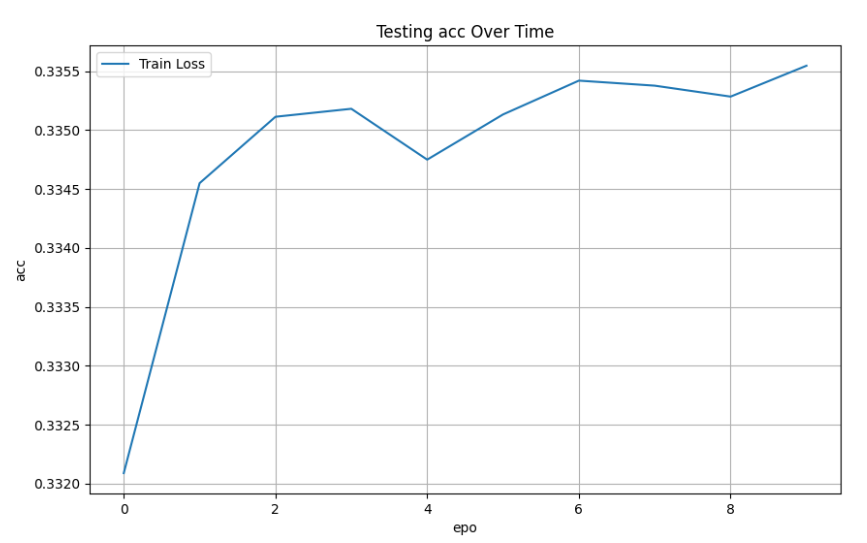
\includegraphics[width=0.9\linewidth]{pictures/accwp.png}
    \end{minipage}
    %\qquad
    \begin{minipage}{0.49\linewidth}
      \centering
      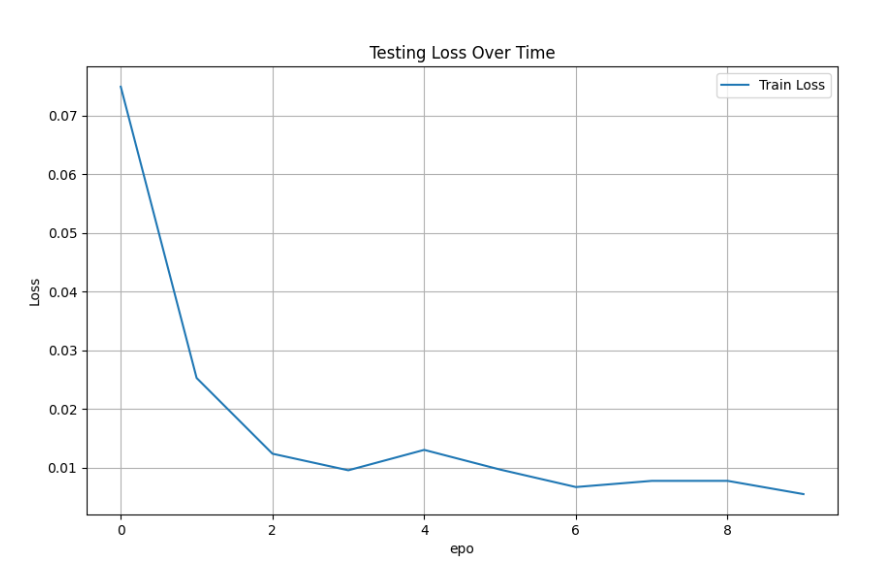
\includegraphics[width=0.9\linewidth]{pictures/losswp.png}
    \end{minipage}
  \end{figure}
\end{frame}

\section{Further steps to be taken}
\begin{frame}
  Old tech: change the parameter used, like learning rate and batchsize;
  
  New tech: DEBERTA V3\cite{he2023debertav3improvingdebertausing}
  \begin{enumerate}
    \item improves the original DeBERTa model by replacing mask language modeling (MLM) with replaced token detection (RTD), a more sample-efficient pre-training task;
    \item not yet updated in text classification task.
  \end{enumerate}
  \begin{figure}[H]
    \centering
    \includegraphics[width=11cm]{D:/Pictures/Screenshots/屏幕截图 2024-07-07 205737.png}
  \end{figure}
\end{frame}
% \begin{frame}
%   %\frametitle{}
%   \begin{figure}[H]
%     \centering
%     \includegraphics[width=10cm]{pictures/}
%     % \caption{}
%   \end{figure}
% \end{frame}
\begin{frame}[allowframebreaks]{Bibliography}
  \bibliography{cite.bib}
\end{frame}
\end{document}